%%%%%%%%%%%%%%%%%%%%%%%%%%%%%%%%%%%%%%%%%%%%%%%%%%%%%%%%%%%%%%%%%%%%%%%%%%%%%%%%%%%%
% Document data
%%%%%%%%%%%%%%%%%%%%%%%%%%%%%%%%%%%%%%%%%%%%%%%%%%%%%%%%%%%%%%%%%%%%%%%%%%%%%%%%%%%%
\documentclass[12pt]{article} %report allows for chapters
%%%%%%%%%%%%%%%%%%%%%%%%%%%%%%%%%%%%%%%%%%%%%%%%%%%%%%%%%%%%%%%%%%%%%%%%%%%%%%%%%%%%
\usepackage{preamble}
\newcommand{\vecx}{\boldsymbol{\vec{x}}}
\newcommand{\vecy}{\boldsymbol{\vec{y}}}

\begin{document}

\begin{center}
   \textsc{\large MATH 271, Homework 11}\\
   \textsc{Due November 22$^\textrm{nd}$}
\end{center}
\vspace{.5cm}

\begin{problem}
A matrix in the group of rotation matrices in $\R^2$ (i.e., $\mathrm{SO}(2)$) can be written as
\[
\Rot_\theta = \begin{pmatrix} \cos \theta & - \sin \theta \\ \sin \theta & \cos \theta \end{pmatrix},
\]
for any choice of $\theta$. Another way to think about $\mathrm{SO}(2)$ is to consider it as the rotational symmetry group of the unit circle in the plane.

Next, consider a cyclohexane $C_6H_{12}$ molecule:
    \begin{figure}[H]
        \centering
        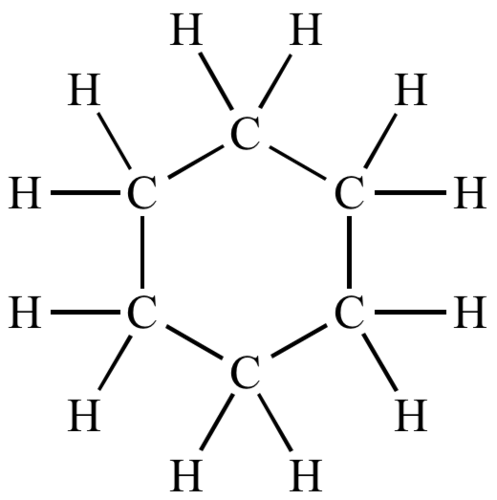
\includegraphics[width=.3\textwidth]{cyclohexane-500x500.png}
    \end{figure}
    \noindent This molecule also has rotational symmetry, but it is a smaller symmetry group than $\mathrm{SO}(2)$. We want to determine this rotational symmetry \emph{subgroup}.
\begin{enumerate}[(a)]
    \item This molecule looks much like a hexagon. Determine the external angles of a hexagon.
    \item Note that if we rotate a hexagon (or cyclohexane) by an external angle, then this leaves the molecule invariant (i.e., it looks no different). Using the internal angle you found, write the rotation matrix for that angle and name this matrix $[g]$.
    \item We can \emph{generate} this group $C_6$ from $[g]$ by repeatedly multiplying $[g]$ with itself.  Show that there are only six elements in this group $C_6$.
    \item These are not all the symmetries of cyclohexane! Explain another symmetry operation that we could use that isn't captured by the rotations above.
\end{enumerate}
If you're interested, look up the group $D_{12}$ which is the \emph{dihedral group of order 12}. Or, taking it further, look at \url{https://en.wikipedia.org/wiki/Cyclohexane_conformation}
\end{problem}


\newpage
\begin{problem}
A matrix in the group of rotation matrices in $\R^2$ (i.e., $\mathrm{SO}(2)$) can be written as
\[
\Rot_\theta = \begin{pmatrix} \cos \theta & - \sin \theta \\ \sin \theta & \cos \theta \end{pmatrix},
\]
for any choice of $\theta$. Another way to think about $\mathrm{SO}(2)$ is to consider it as the rotational symmetry group of the unit circle in the plane.

Next, consider a cyclohexane $C_6H_{12}$ molecule:
    \begin{figure}[H]
        \centering
        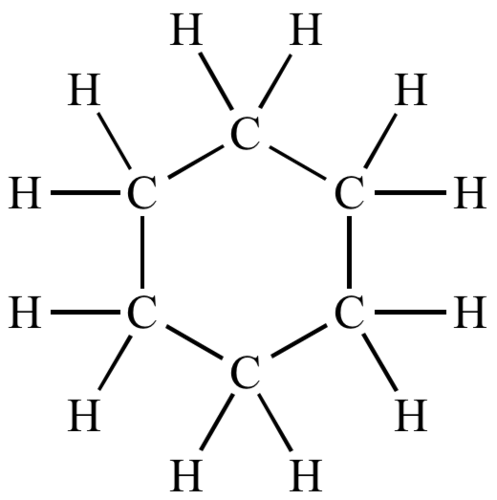
\includegraphics[width=.3\textwidth]{cyclohexane-500x500.png}
    \end{figure}
    \noindent This molecule also has rotational symmetry, but it is a smaller symmetry group than $\mathrm{SO}(2)$. We want to determine this rotational symmetry \emph{subgroup}.
\begin{enumerate}[(a)]
    \item This molecule looks much like a hexagon. Determine the external angles of a hexagon.
    \item Note that if we rotate a hexagon (or cyclohexane) by an external angle, then this leaves the molecule invariant (i.e., it looks no different). Using the external angle you found, write the rotation matrix for that angle and name this matrix $[g]$.
    \item We can \emph{generate} this group $C_6$ from $[g]$ by repeatedly multiplying $[g]$ with itself.  Show that there are only six elements in this group $C_6$.
    \item These are not all the symmetries of cyclohexane! Explain another symmetry operation that we could use that isn't captured by the rotations above.
\end{enumerate}
If you're interested, look up the group $D_{12}$ which is the \emph{dihedral group of order 12}. Or, taking it further, look at \url{https://en.wikipedia.org/wiki/Cyclohexane_conformation}
\end{problem}
\begin{solution}~
\begin{enumerate}[(a)]
    \item The external angles of a hexagon are $\pi/3$ since the sum of the external angles must be $2\pi$ and there are six angles on a hexagon.
    \item Then we have
    \[
    [g]=\begin{pmatrix} \sqrt{3}/2 & -1/2 \\ 1/2 & \sqrt{3}/2 \end{pmatrix}.
    \]
    \item Now, we can explicitly compute $[g]$, $[g]^2$, $[g]^3$, and so on, but remember that this is a rotation matrix.  Hence, for example, we have
    \[
    \Rot_\theta \Rot_\varphi = \Rot_{\theta+\varphi}.
    \]
    Hence, we have
    \[
    [g]^2 = \Rot_{\pi/3},\quad [g]^3 = \Rot_{\pi/2}, \quad [g]^4 = \Rot_{2\pi/3}, \quad [g]^5 = \Rot_{5\pi/6}, \quad [g]^6 = \Rot_{2\pi}=[I].
    \]
    Indeed, this group does have six elements as there is no way to create any others. This group is known as the \emph{cyclic group of order 6} and we denote it by $C_6$.
    \item The cyclohexane molecule also has reflectional symmetry. That is, we could pick up the molecule, and flip it over (across some axis) and place it back in the same spot. If we include this symmetry as well, we can then generate $D_{12}$. 
\end{enumerate}
\end{solution}

\begin{remark}
The groups $C_n$ and $D_{2n}$ always have this same relationship as the groups $\Orth(n)$ and $\SO(n)$. The idea of rotations and reflections are very related. In fact, reflections are more fundamental in that any rotation is a product of two reflections. This is exactly why we see this relationship.

Also, $\Orth(n)$ and $\SO(n)$ give the reflection/rotation symmetries of $n$-dimensional space. However, we can see that some objects living in those spaces will have smaller symmetry groups. In this case, the group is even finite (order 6) as opposed to infinite!
\end{remark}
\end{document}